\documentclass[a4paper, 11pt]{article}
\usepackage[utf8]{inputenc}
\usepackage[hyphens]{url}
\usepackage[slovak]{babel} 
\usepackage{cite}

\usepackage[left=2cm,text={17cm, 24cm},top=3cm]{geometry}
\usepackage{times}
\usepackage{amsmath}
\usepackage{amsthm}
\usepackage{amsfonts}
\usepackage{textcomp}
\usepackage{multirow}
\usepackage[ruled,longend,linesnumbered]{algorithm2e}
\usepackage{graphicx}
\graphicspath{ {./images/} }
\usepackage{pict2e}
\usepackage{wrapfig}

\usepackage[unicode=true,hidelinks]{hyperref}
\usepackage{epstopdf}
\hypersetup{breaklinks=true}

%\addto\captionsslovak{\renewcommand*\contentsname{Obsah}}

\begin{document}
\begin{titlepage}
    \begin{center}
        {\Huge\textsc{Vysoké učení technické v Brně}}\\[0.4em]
        {\huge\textsc{Fakulta informačních technologií}}\\
        \vspace{\stretch{0.382}}
        {\LARGE Modelování a simulace}\\[0.3em]
        {\Huge Model pomocí celulárního automatu}\\
        \vspace{\stretch{0.618}}
    \end{center}
        {\Large \hfill
        Adam Fabo (xfaboa00) \\ 12. decembra 2021 \hfill Stanislav Gabriš (xgabri18)}
\end{titlepage}

\tableofcontents

\pagebreak 

\section{Úvod}
% V prírode dochádza k mnoho zaujmavím javom, medzi nimi je aj synchronizácia. My sme sa v našom projekte rozhodli skúmať práve tento jav spontánnej synchronizácie blikania pri svetluškách Photinus carolinus.

% Je to fascinujúce, že v prírode dochádza k spontánnej synchronyzácii. A my robime svetlusky.

Druhý termodynamický zákon hovorí, že všetko vo vesmíre inklinuje ku chaosu\cite{Thermo} a v komplexných systémoch (three body problem, double pendulum) je chaos normou. Podľa tohto tvrdenia by sa dalo očakávať, že vesmír bude chaotický a neusporiadaný. Ale aj tak môžeme pozorovať javy spontánnej synchronizácie, ako napríklad synchronizáciu metronómov, viazanú rotáciu nebeských telies alebo zladené blikanie svetlušiek na strome.\cite{Svetlusky}\cite{Strogatz} Ako je možné, že aj napriek vlastnostiam vesmíru v ktorom žijeme, je možné pozorovať takéto fascinujúce úkazy? 

% https://sciencedemonstrations.fas.harvard.edu/presentations/synchronization-metronomes
% https://en.wikipedia.org/wiki/Second_law_of_thermodynamics
% https://en.wikipedia.org/wiki/Double_pendulum
% https://en.wikipedia.org/wiki/Tidal_locking
% https://www.nytimes.com/2021/07/07/science/fireflies-sync-flashes.html

Táto simulačná štúdia sa zaoberá zladeným blikaním svetlušiek \textit{Pteroptyx malaccae}, ktoré pochádzajú z~Thajských lesov. Tieto svetlušky majú v určitom okolí schopnosť zosynchronizovať sa tak, aby všetky blikali naraz aj napriek rozličným počiatočným frekvenciam blikania. Simulačný model je koncepovaný na štýl celuárneho automatu, ktorý sa opiera o základy synchronizácie, ktoré položil pán Kuramoto v roku 1975\cite{Kuramoto2}. Model, ktorý tu je prezentovaný, je rozšírením Kuramoto modelu (\ref{kuramoto_eq}) o rôzne charakteristiky svetlušiek, ktoré, dúfajúc, môžu poskytnúť dodatočné informácie o tom ako a kedy dochádza k synchronizácii svetlušiek.

% https://en.wikipedia.org/wiki/Kuramoto_model#cite_note-1
% https://link.springer.com/content/pdf/10.1007/BF00164052.pdf

V kapitole \ref{sec_facts} je vysvetlenie základnej formy Kuramoto modelu a klasifakácie a charakteristiky synchronizácie viazaných oscilátorov, ktoré sú využívané v neskorších kapitolách. Tretia kapitola sa zaoberá prezentovaním koncepcie 
modelu tejto simulačnej štúdie. Tu je možné dočítať sa o rozšíreniach pôvodného modelu a~jeho zakomponovanie do celuárneho automatu. Štvrtá kapitola sa zaoberá experimantami ktorých zmyslom je v prvom rade zistiť, či ide modelovať synchronizáciu svetlušiek pomocou celuárneho automatu a demonštrovať synchronizáciu pri rôznych počiatočných podmienkach. V poslednej kapitole je~môžné sa dočítať o závere tejto modelačnej štúdie.














\pagebreak 
\section{Fakty} \label{sec_facts}
%synchronizacia happens
%svetlusky su schopne synchronizacie
%rozne mechanizmi synchronizacie
%svetlo sa siri pomocou zakonu prevratenych stvorcov
%what else?
%svetlusky a co a ako, vilo rozboril, kuramoto model to ma pokryte
%osci,order, 2d rovina


Synchronizácia sa v prírode naturálne vyskytuje. Či už pri synchronizácii tlieskania davu, synchronizácii\\ metronómov alebo v neposlednom rade pri blikaní svetlušiek. \cite{Svetlusky}\cite{Strogatz}\cite{Kuramoto2}


%toto pojde do koncepcie
\vspace{1em}
\noindent
Hlavná rovnica Kuramoto modelu synchronizácie\cite{Strogatz}\cite{Kuramoto2}
\begin{equation} \label{kuramoto_eq}
    \theta_i = \omega_i + \frac{K}{N} \sum_{j=1}^{N} \sin(\theta_j - \theta_i), \hspace{1em} i = 1,\dots, N
\end{equation}

Tento model pozostáva z \textit{N} vzájomne rovnako viazaných oscilátorov so svojou vlastnou vnútornou\\ frekvenciou ($\omega$). Tieto frekvencie sú distribuované podľa nejakej pravdepodobnostnej funkcie. \textit{K} $\geq 0$ udáva silu viazanosti oscilátorov a $1/$\textit{N} usmerňuje model pre \textit{N} $\to\infty$.\cite{Strogatz}

Kuramoto model je netriviálny, dokáže ukázať rôzne synchronizáčné vzory a je dostatočne flexibliný\\ aby sa dal adaptovať do rôznych situácií \cite{Kuramoto2}, ako napríklad synchronizácia svetlušiek.

\vspace{1em}
\noindent 
Svetlušky sú schopné synchronizácie vďaka malým úpravám svojho cyklu blikania. \cite{Svetlusky}\cite{NatGeoSvetlusky} Rôzne druhy svetlušiek využívajú rôzne mechanizmi na dosiahnutie tohtu javu a to urýchlenie fázového posunu, oneskorenie fázového posunu alebo ako v prípade druhu \textit{Pteroptyx malaccae} perfektnú synchronizáciu.\cite{Svetlusky}

\vspace{1em}
\noindent 
Zákon prevrátených štvorcov hovorí, že intenzita svetla klesá s druhou mocnicou vzdialenosti od zdroja. \cite{InverseLaw} Pre výpočet intenzity v 2-dimenzionálnom priestore:
\begin{equation} \label{inverse_eq}
    \frac{1}{\sqrt{x^2+y^2}}
\end{equation}



%v našom prípade to je normálne rozdelenie.

%ej ty tu nieco robis - uz som dokoncil vsetko aj video and stuff a zajtra zacnem pisat toto 
%video ? do pdf?










\pagebreak 
\section{Koncepcia}
Model synchronizácie svetlušiek sa dá koncpipovať ako model synchronizácie previazaných oscilátorov. Svetluška, ktorá bliká, predáva informácie ostatným svetluškám o svojej frekvencii blikania, ktoré poupravia svoju frekvenciu blikania tak aby bola bližšie k frekvencii svetlušky ktorej svetlo zaregistrovali. Takýmto spôsobom je možné, že po určitom čase budú všetky svetlušky blikať naraz \cite{NatGeoSvetlusky}. Model synchronizácie, na ktorom je postavená táto simulačná štúdia sa nazýva Kuramoto model.

\subsection{Kuramoto model}

Základný Kuramoto model (\ref{kuramoto_eq}) robí niekoľko predpokladov \cite{Kuramoto2}. Medzi ne patrí predpoklad, že sa všetky oscilátory ovplivňujú v každom kroku a predpoklad, že sila akou sa ovplivňujú je rovnaká medzi všetkými oscilátormi. Tento model je názorne ukázaný na správaní sa viacerých metronómov, každý s inou fázou, na pohyblivom podklade\footnote{Video ukazujúce synchronizáciu metronómov:
\href{https://www.youtube.com/watch?v=Aaxw4zbULMs}{https://www.youtube.com/watch?v=Aaxw4zbULMs}.}. Po určitom čase je možné pozorovať zosynchornyzovanie metronómov.
%Tento model dokáže opísať napríklad s

\begin{figure}[h]
    \hspace*{-0.8cm}
    %\vspace*{-2cm}
    \resizebox{18cm}{12cm}{\includegraphics{images/kuramoto.eps}}
\caption{Kuramoto model\label{obr1}}
\end{figure}


% Na obrázku \ref{obr1} je možné vidieť niekoľko vlastností systému oscilátorov pri Kuramoto modeli (\ref{kuramoto_eq}). V ľavom hornom rohu je možné vidieť ako sa oscilátory postupom krokov synchronizujú. V pravom hornom rohu graf opisuje vlastnosť zvanú \textit{Poriadok}, táto naberá hodnotu v rozmedzí 0 až 1, kde 1 znamená najväčší poriadok. \textit{Poriadok} ukazuje ako dobre zosynchronizovaný je systém oscilátorov postupom krokov, a teda ideálny poriadok je 1. Táto hodnota sa vypočíta podľa vzorca \ref{vectorlength_eq}. Ak zakreslíme priebeh oscilátorov do komplexnej roviny, a zoberieme súčet vektorov, ktorý znormalizujeme, dostaneme vektor znázorňujúci \textit{Poriadok}. Na výpočet súradníc tohto vektora teda slúžia vzorce \ref{order_eq}. \cite{KuramotoCycle} 


Na obrázku \ref{obr1} je možné vidieť niekoľko vlastností systému oscilátorov pri Kuramoto modeli (\ref{kuramoto_eq}). V ľavom hornom rohu je možné vidieť ako sa oscilátory postupom krokov synchronizujú. Ak zakreslíme priebeh oscilátorov do komplexnej roviny, a zoberieme súčet vektorov, ktorý znormalizujeme, dostaneme vektor znázorňujúci \textit{Poriadok}. \textit{Poriadok} ukazuje ako dobre zosynchronizovaný je systém oscilátorov postupom krokov, a teda ideálny poriadok je 1. Na výpočet súradníc tohto vektora teda slúžia vzorce \ref{order_eq} \cite{KuramotoCycle}. V pravom hornom rohu graf ukazuje absolútnu hodnotu \textit{Poriadku} vypočítanú podľa vzorca \ref{vectorlength_eq}. Toto bude hlavná metrika merania synchronizácie systému v modeli.


\begin{equation} \label{order_eq}
    x =  \frac{1}{N} \sum_n cos(\theta_n), \hspace{2em}  y =  \frac{1}{N} \sum_n sin(\theta_n) 
\end{equation}

\begin{equation} \label{vectorlength_eq}
    poriadok = \sqrt{x^2 + y^2} 
\end{equation}





% Pre potreby tohto projektu, bol základný Kuramoto model (\ref{kuramoto_eq}) upravený aby odpovedal situácii zo svetluškami.

% V prvom rade, ako je opísane v sekcii \ref{Ovplivnovanie}, sa svetlušky ovplivňujú len ak niektorá z nich zabliká, narozdiel od toho aby sa ovplivňovali v každom kroku, ako prepokladá základný Kuramoto model (\ref{kuramoto_eq}). Táto skutočnosť sa prejavý vo vzorci úpravou sumy sínusov





\subsection{Rozšírenie o blikanie svetlušky} \label{Ovplivnovanie}
Model, ktorý tu je prezentovaný sa lýši od modelu v štúdii o ktorú sa táto modelačná štúdia opiera \cite{Svetlusky}. Ako je možné vidieť v kuramoto modeli (\ref{kuramoto_eq}), tak všetky oscilátory (svetlušky) sa ovplyvňujú v každom kroku. Tento predpoklad ale nie je pravdivý, pretože svetluška získava informácie iba ak registruje bliknutie inej svetlušky.

%(pilka here)
\begin{figure}[h]
    \vspace*{-0.2cm}
    \centering
    \scalebox{0.45}{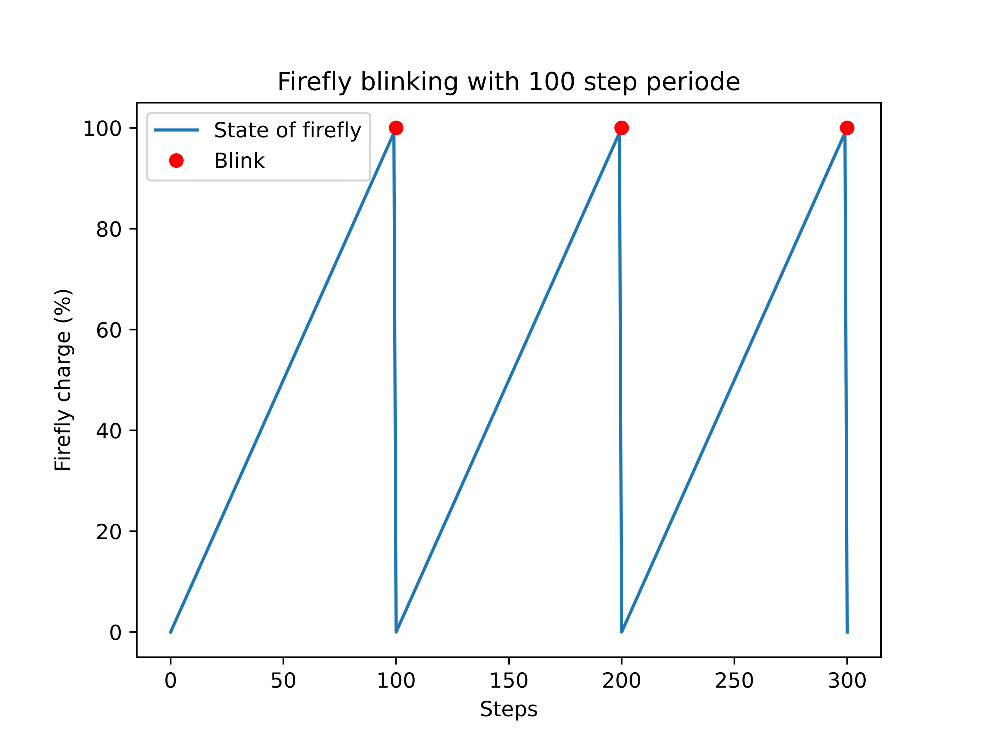
\includegraphics{pilka}}
\caption{Blikanie svetlušky\label{pilka}}
\end{figure}

Možno ide tento fakt zanedbať, ale v rámci rozšírenia pôvodnej štúdie sme sa rozhodli zakomponovať aj~tento poznatok. Na obrázku \ref{pilka} je možné vidieť priebeh blikania jednej svetlušky, pričom svetluška blikne až po čase nabitia, pričom dĺžka nabitia je daná jej vnútorným oscilátorom. Keď svetluška blikne, tak sa vybíja a~cyklus sa opakuje. 

\subsection{Rozšírenie o váhovanie svetlušiek} \label{sec_vahovanie}
Ďaľším rozdielom je riešenie väzby medzi oscilátormi. V Kuramoto modeli (\ref{kuramoto_eq}) sa všetky viazané oscilátory ovplyvňujú navzájom rovnakou silou. Keďže svetlušky v realite majú medzi sebou nenulové vzdialenosti a~spôsob synchronizácie medzi nimi prebieha pomocou svetla, tak je možné modelovať aj rozptyl tohto svetla v priesore. Ako je možné vedieť z fyziky, tak intenzita svetla (energie) klesá druhou mocninou vzdialenosti od zdroja.\cite{InverseLaw} 
%(mozno rovnica?)
%(inverse pic here)
\begin{figure}[h]
    \vspace*{-0.9cm}
    %\resizebox{18cm}{12cm}{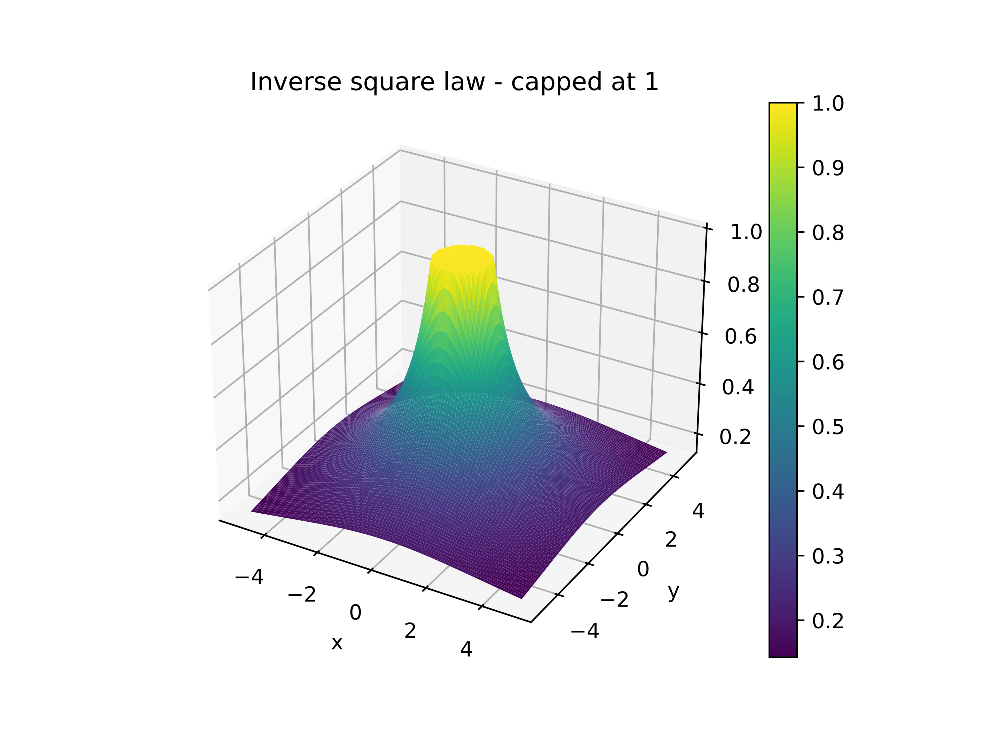
\includegraphics{inverse}}
    \centering
    \scalebox{0.5}{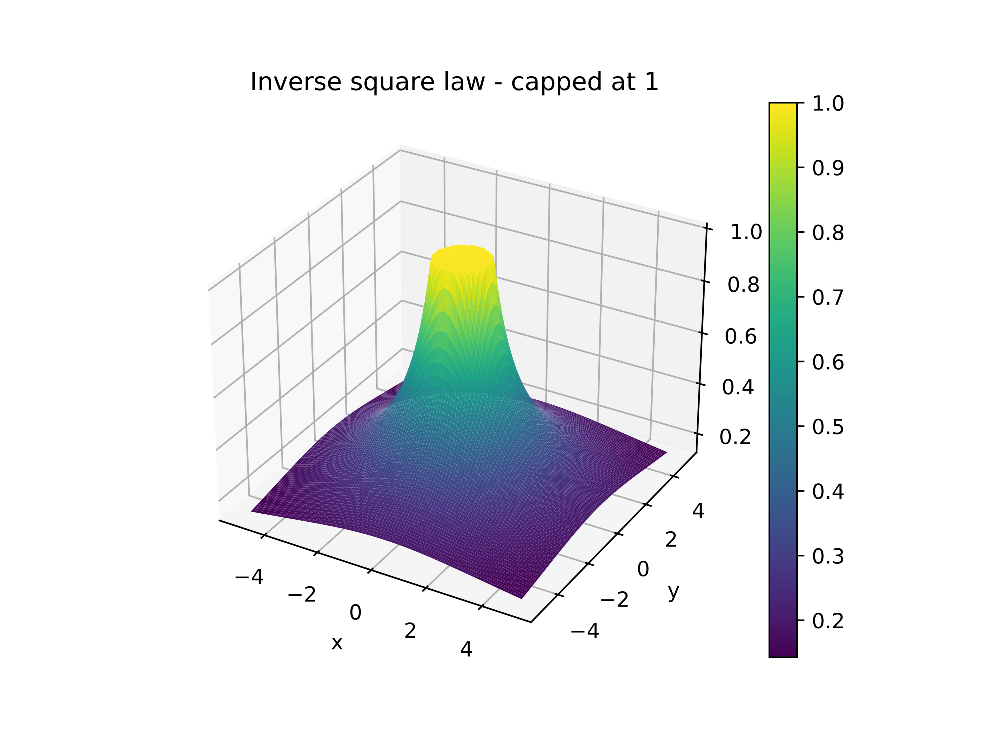
\includegraphics[height=11cm]{inverse}}
\caption{Graf zákonu prevrátených štvorcov\label{Inverse}}
\end{figure}

\pagebreak
V modeli svetlušky vedia určiť koľko svetla na ne dopadlo a podla toho upraviť svoju frekvenciu blikania (čím je zdroj svetla silnejší/bližšie tým viacej svetluška upraví svoju frekvenciu blikania). Hoci je toto modelovanie fyzikálne správne, znamemalo by to že v nulovej vzdialenosti je intenzita nekonečná. Z tohoto dôvodu je intenzita limitovaná hodnotou 1 ako je možné vidieť na obrázku \ref{Inverse}. 
%Toto ohraničenie môže taktiež z pohľadu svetlušky ktorá prijíma toto svetlo znamenať že jej receptory na registrovanie svetla sú na maxime svojej kapacity a nedokážu už rozlýšiť intenzitu svetla

% Ďaľší rozdiel je ten, že v kuramoto modeli (\ref{kuramoto_eq}) sa ovplivňujú všetky oscilátory navzájom. To taktiež v modeli so svetluškami nemusí byť pravda, keďže medzi svetluškami sú nenulové vzdialenosti. Ako je možné vedieť z fyziky(citacia here) svetlo sa v priestore podľa invrse square law. Tento zákon vraví, že energia vyžarovaná zo zdroja, ktorá dopadne na jednotku plochy  je nepriamo úmerná vzdialenosti na druhú. V modeli sa snažíme zakomponovať túto skutočnosť a to tak že svetluška upraví svoj vnútorný oscilátor v priamej úmere podľa toho, koľko svetla na ňu dopadne. - opisat capped at one? -- 

% (insert picture here) to co je pod tymto mozno do fakta
\subsection{Návrat k vnútornej frekvencii} \label{sec_backtofreq}
Ako je možné vidieť z kuramoto modelu (\ref{kuramoto_eq}), má každá svetluška svoju vlastnú vnútornú frekvenciu $\omega_{nat}$ podľa ktorej bliká. V prípade externého stimulu (svetla z iných svetlušiek) sa však táto frekvencia mení. Ako sa zachová frekvencia blikania svetlušky, ak prestane registrovať blikanie ostatných svetlušiek?
Podľa štúdie na~ktorej je táto simulačná šudia založená \cite{Svetlusky}, sa svetluška postupne vracia ku svojej pôvodnej frekvencii blikania podľa nasledujúceho vzorca:
\vspace{1em}
\begin{equation} \label{damping_eq}
   \omega_{next} = \varepsilon(\omega_{nat} - \omega)
\end{equation}
kde $\omega_{nat}$ predstavuje pôvodnú frekvenciu, $\omega$ súčasnú frekvenciu a $\varepsilon$ rýchlosť akou sa oscilátor (svetluška) vracia k pôvodnej frekvencii. \cite{Svetlusky}

%(drop image freq to norm here)
\begin{figure}[h]
    \centering
    \scalebox{0.4}{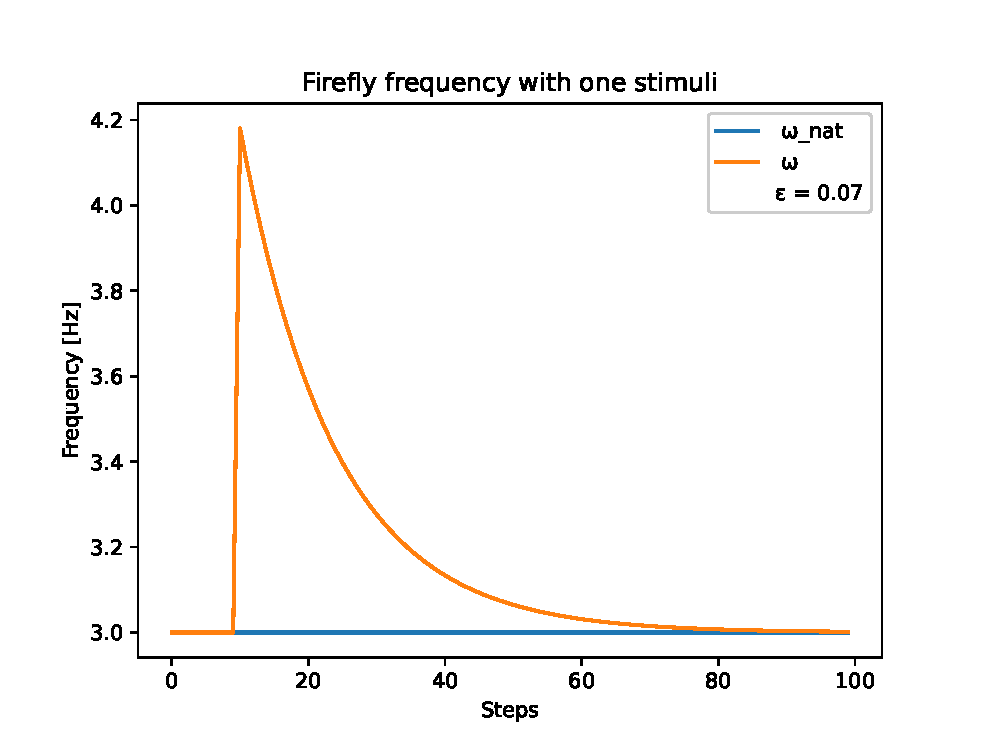
\includegraphics{freq_to_norm}}
\caption{Návrat frekvencie k $\omega_{nat}$\label{ToNorm}}
\end{figure}

Na obrázku \ref{ToNorm} je vidieť možný graf priebehu navrátenia frekvencie svetlušky pri jednorazovom externom stimuli.


\subsection{Zakomponovanie do celulárneho automatu} \label{sec_celular}

Model celuárneho automatu pozostáva z 2-dimenzionálneho pola buniek, pričom každá bunka predstavuje jednu svetlušku. Každá bunka má v sebe uloženú vlastnú frekvenciu blikania, fázový posun a môže nadobudnúť jeden zo stavov \texttt{svieti/nesvieti}. Do stavu \texttt{svieti} sa dostane po uplinutí jednej periódy, tento stav si zachová po dobu jedného kroku simulácie. Počas tohto kroku ovplivní frekvencie blikania okolitých svetlušiek, ako je znázornené v \ref{alg1}, a následne svetluška mení stav na \texttt{nesvieti}.

\vspace{1em}
\begin{algorithm}[h]
\DontPrintSemicolon
\SetAlgorithmName{Algoritmus}
% space necessary

\Indp
\SetNlSty{}{}{}
    \For{Každá svetluška}{
        \If{Svetluška zasvietila}{
            Ovplivni ostatné svetlušky
        }
        
    }
\caption{\textsc{Krok\,-\,Ovplivnenie}\label{alg1}}     
\end{algorithm}

\subsection{Okolie bunky}
% \begin{wrapfigure}{r}{0.25\textwidth} %this figure will be at the right
%     \centering
%     \vspace*{-1cm}
%     \hspace*{-0.5cm}
%     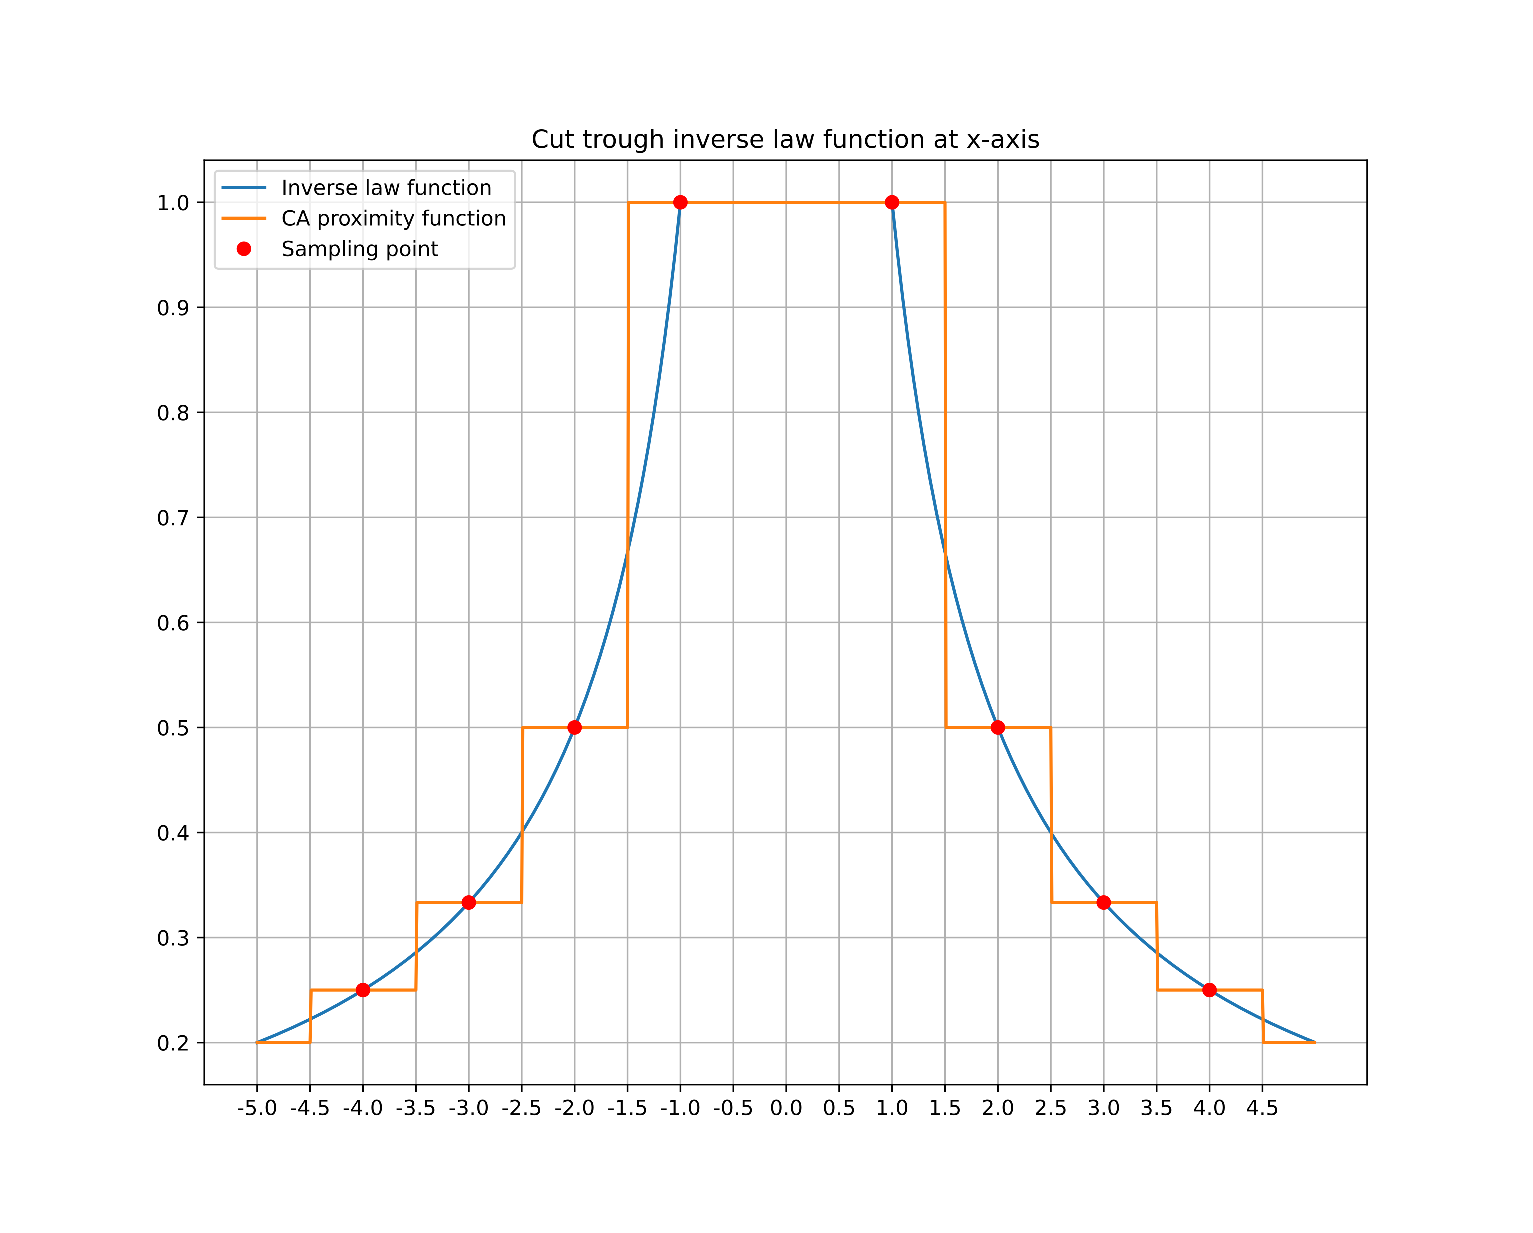
\includegraphics[width=0.4\textwidth]{okolie}
% \end{wrapfigure}

Z priamočiarého pohľadu má bunka nekonečné okolie, t.j. každá bunka má dosah na každú bunku. Čo je ale podstatné na okolí bunky sú koeficienty priradené každej bunke jej okolia. Koeficienty vychádzajú už zo spomenutého zákona prevrátených štvorcov. Lenže funkcia popisujúca tento fyzikálny jav je spojitá a treba ju namapovať na funkciu okolia bunky.



Výpočet koeficientu prebieha jednoduchým spôsobom. Najprv sa vypočítajú relatívne vzdialenosti oboch svetlušiek na x a y ose a tieto hodnoty sa dosadia do vzorca \ref{inverse_eq}.



\begin{figure}[ht]
    \centering
    \scalebox{0.6}{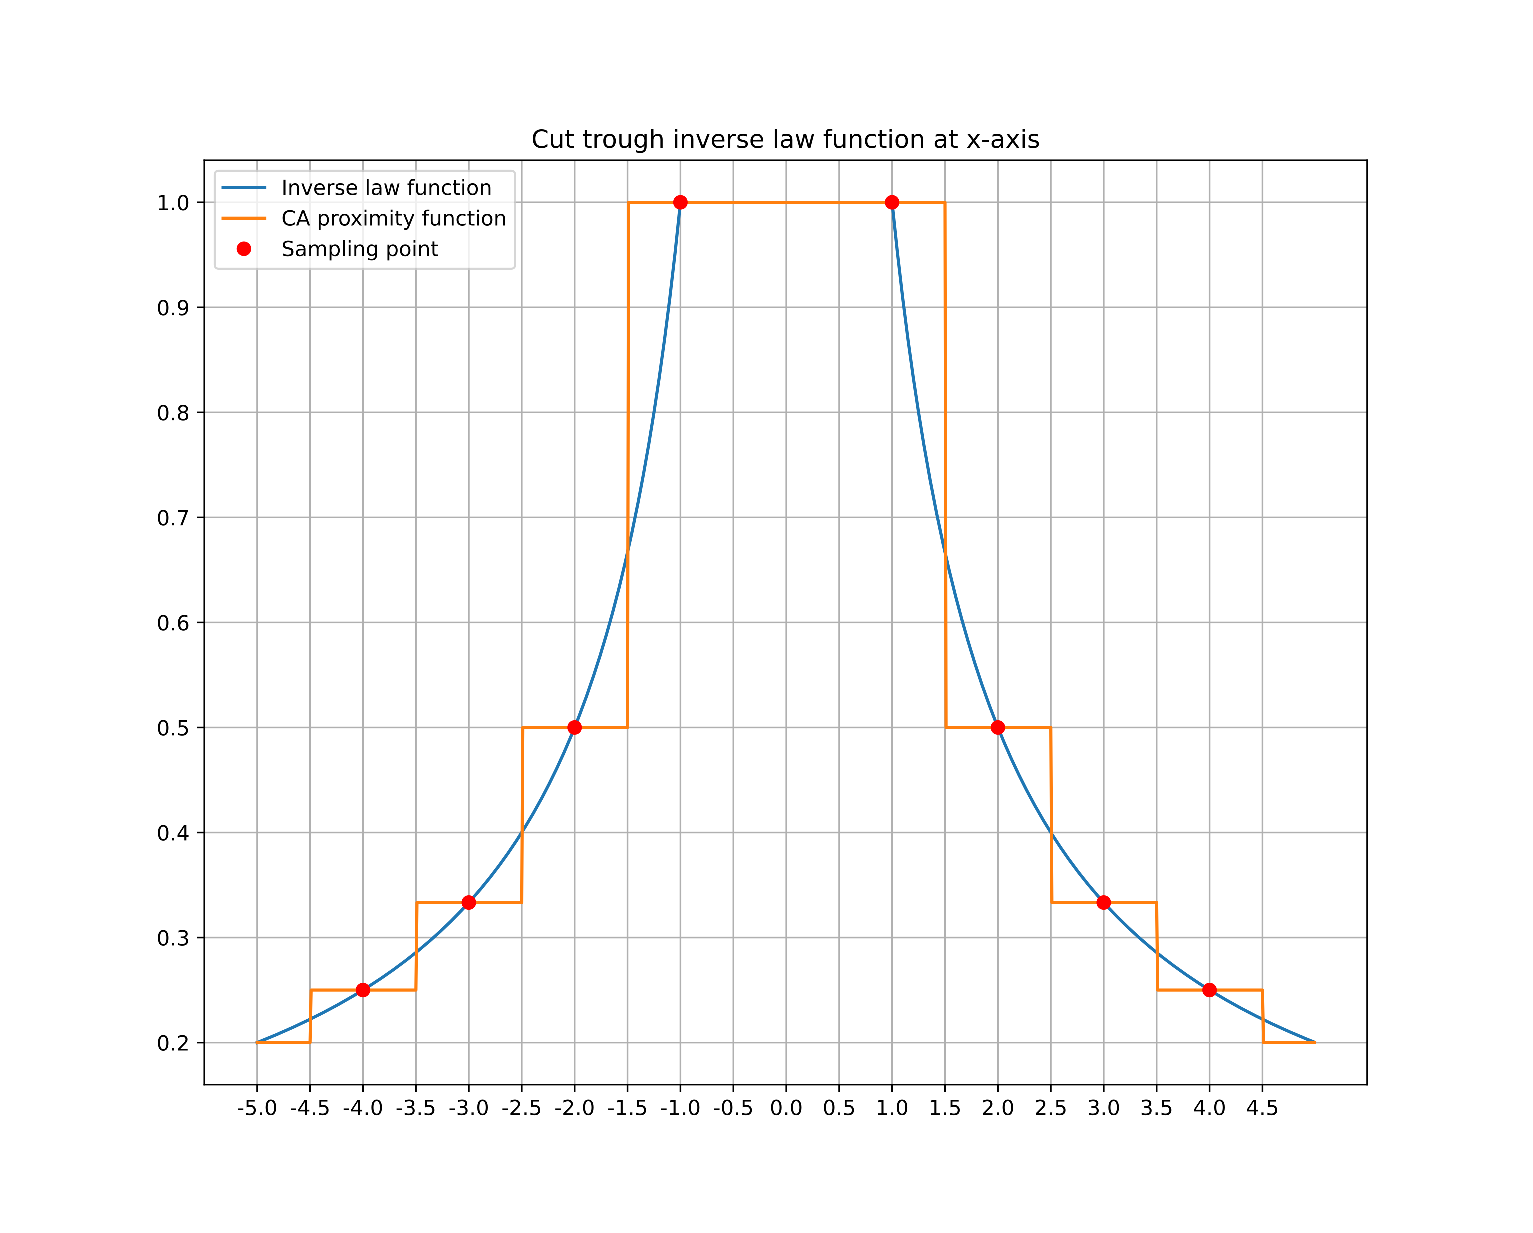
\includegraphics{okolie}}
\caption{Okolie\label{Okolie}}
\end{figure}

Obrázok \ref{Okolie} ilustruje rez funkciou na x-ovej ose a namapovanie vypočítanej hodnoty zo stredu bunky svetlušky na celú jednotkovú dĺžku.

\pagebreak


\subsection{Synchronizácia modelu} \label{sec_synchron}

Vyhodnocovanie úspešnosti synchronizácie prebieha už podľa spomenutého výpočtu poriadku. Pokiaľ sa zoradenosť modelu blíži k jednotke, svetlušky môžeme považovať za úspešne zosynchronizované. Ak sa zoradenosť neblíži k jednotke model sa považuje za nezosynchronizovaný a ak osciluje medzi hodnotami, tak sa považuje za nestabilný.
%(insert order here)
%mozno order nejako zmenit aby tam bol aj koef
Ako príklad je uvedený obrázok \ref{Order} ktorý ukazuje 3 priebehy simulácie, pričom v jednom sú svetlušky nezosynchronizované (graf vľavo), v druhom sú zosynchronizované (graf v strede) a v treťom (graf vpravo) nestabilné.

\begin{figure}[ht]
    \hspace*{-1.1cm}
    \scalebox{0.5}{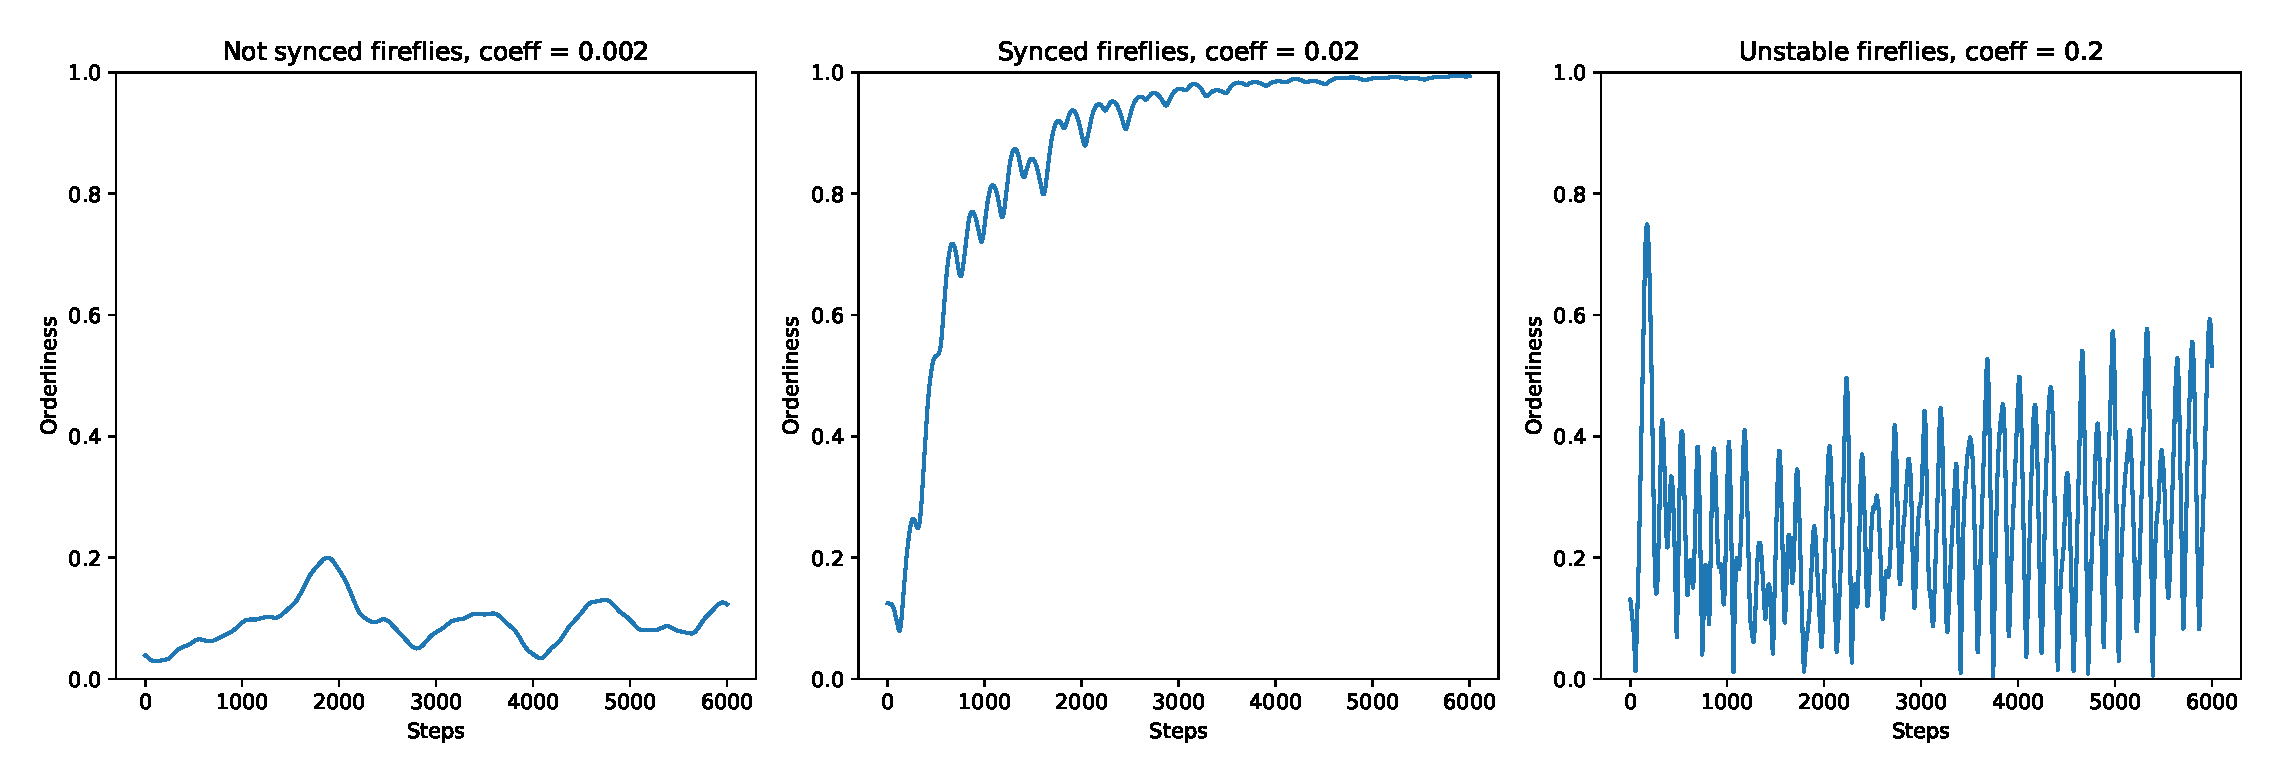
\includegraphics{order}}
\caption{Synchronizácia pri rôznych koeficientoch\label{Order}}
\end{figure}


\subsection{Koeficient viazanosti}
Koeficient viazanosti (ďalej už len koeficient) spomenutý pri vzorci Kuramoto modeleu je hlavným vstupom simulácie. Koeficient hovorí o sile viazanosti medzi oscilátormi, t.j ako moc upraví svetluška svoju frekvenciu pri rozsvietení inej svetlušky. Veľkosť koeficientu značí ako moc ideálne podmienky sú medzi svetluškami. Nízky koeficient môže znamenať napríklad hustú korunu stromu na ktorej svetlušky sedia alebo hmlu ktorá tlmí svetlo vyžarované svetluškami, ale môže znamenať aj veľké vzdialenosti medzi svetluškami. Väčší koeficient značí ideálne podmienky a moc velký koeficient hovorí o prehnanom reagovaní svetlušiek na svetlo.

Ako je možné vidieť na obrázku \ref{Order} simulácie majú rôzne priebehy pričom sa lýšia v koeficiente viazanosti. 


\subsection{Koeficient svitu svetlušky}
Pre zavedenie modelovania svitu svetlušky sa zaviedol do rovnice \ref{inverse_eq} koeficient \textit{m} do čitatela, ktorý hovorí o tom ako silno svetluška svieti. Stále platí, že výstupná hodnota funkcie je limitovaná hodnotou 1, ako je spomenuté v časti \ref{sec_vahovanie}. 





\subsection{Počiatočné hodnoty svetlušiek}
Ako je spomenuté v časti \ref{sec_celular}, tak svetlušky majú v sebe uloženú vlastnú frekvenciu blikania a fázový posun. Keďže žiadne dve svetlušky nie sú rovnaké, tak vlastné frekvencie a počiatočné fázové posuny svetlušiek sú~generované náhodne pomocou normálneho rozdelenia so stredom v hodnote $\mu$ a rozptylom $\sigma$. 



\subsection{Spustenie programu}
Program pozostáva zo súborov \textit{fireflies.h} a \textit{fireflies.cpp}, ktoré popisujú triedu \texttt{svetluška}, a z hlavného súboru \textit{fireflies\_main.cpp}, v ktorom sa nachádza funkcia \texttt{main}. Pre preklad programu slúži súbor \textit{Makefile} a príkaz~make.

Spúšťanie programu má nasledovnú formu: \texttt{fireflies X Y KOEF MI SIGMA}\\ 
kde \texttt{X} a \texttt{Y} udávajú veľkosť pola (množstvo svetlušiek), \texttt{KOEF} udáva silu akou sa svetlušky ovplivňujú. Parametre \texttt{MI} a \texttt{SIGMA} predstavujú strednú hodnotu a rozptyl pri normálnom rozdelení frekvencií medzi svetluškami.


\subsection{Video ukážka synchronizácie svetlušiek}
Názorná ukážka toho ako môže synchronizácia vyzerať. Vľavo je možné vidieť blikanie svetlušiek, pričom pre lepšie znázornenie im bola pridaná zotrvačnosť blikania (v simulácii blikajú len po dĺžku jedného kroku). Vpravo je môžné vidieť priebeh synchronizácie simulácie, pričom na začiatku svetlušky blikajú chaoticky a~postupne sa dostávajú do jednotného blikania. Video má približne 1 min a je ho možné nájsť na Youtube (\href{https://youtu.be/UF8tPC8jpdA}{\textbf{Link}}) alebo na Google Drive (\href{https://drive.google.com/file/d/1B7llCROASMtfPk-YtsiF4w4MxkObrWJH/view?usp=sharing}{\textbf{Link}})



%(snimka obrazovky here potom)

% \begin{figure}[ht]
%     \hspace*{-1.1cm}
%     \scalebox{0.5}{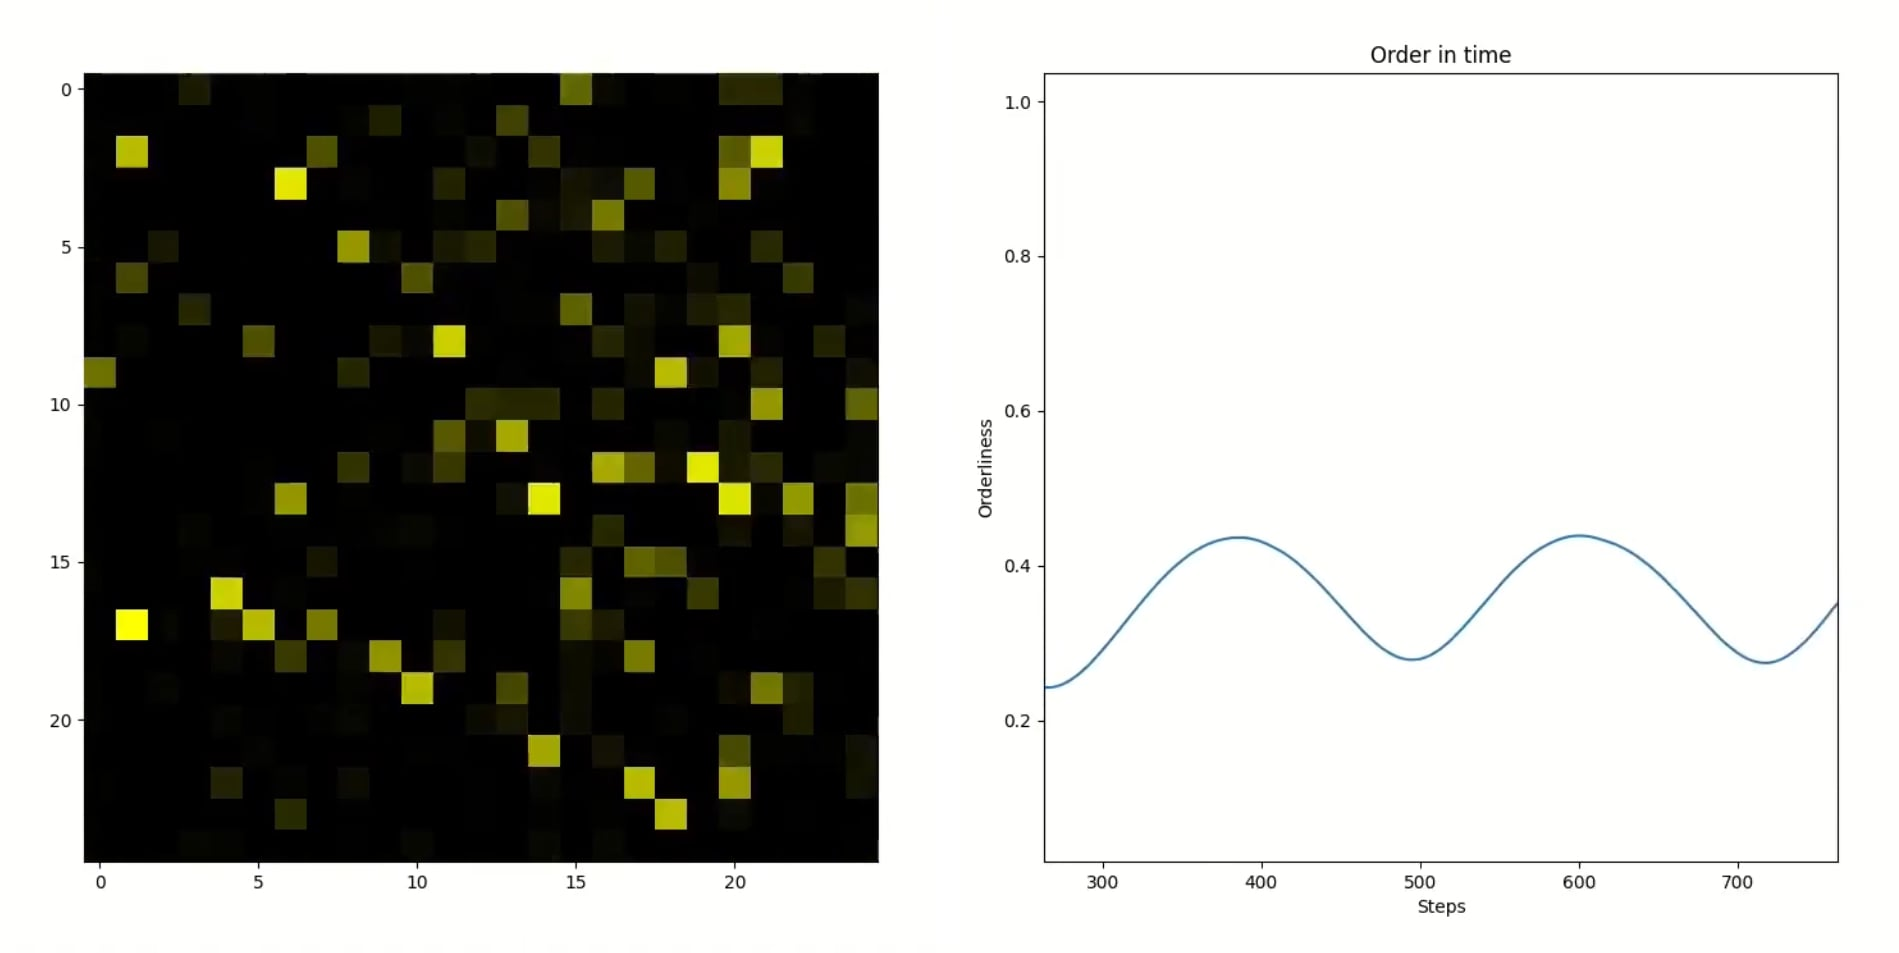
\includegraphics{obr}}
% \caption{Poriadok\label{video}}
% \end{figure}

\begin{figure}[h]
\centering
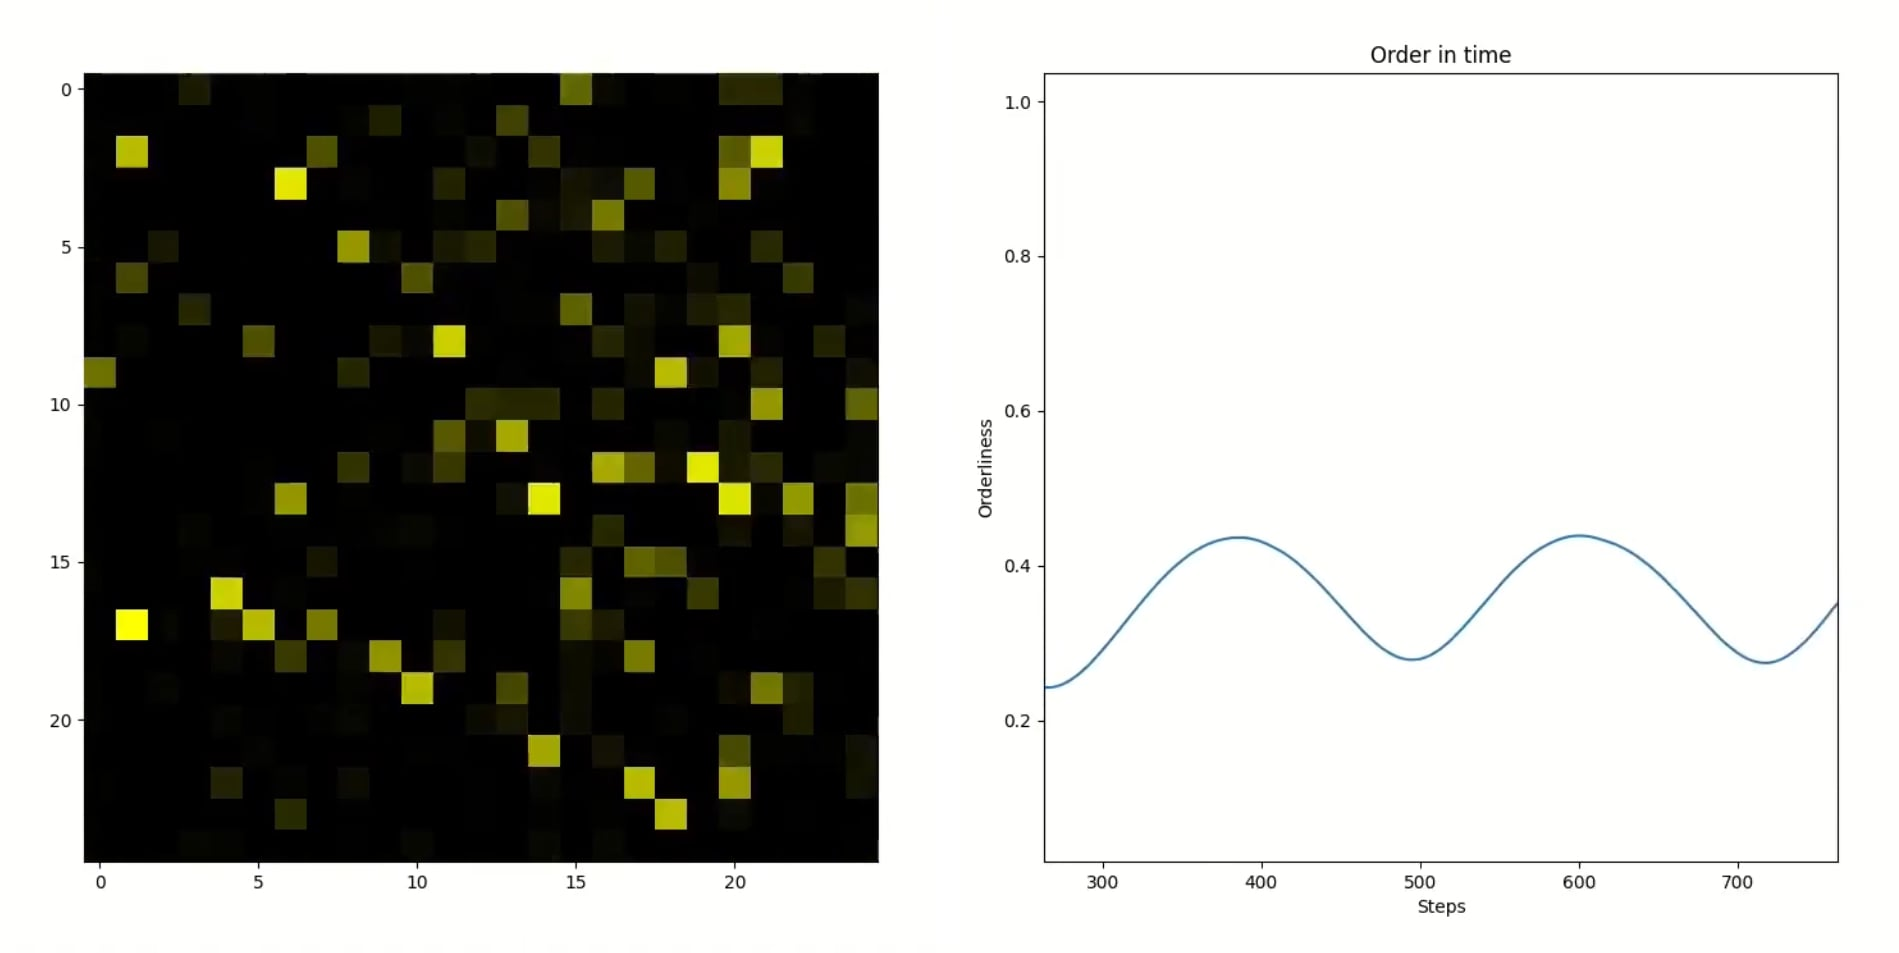
\includegraphics[width=15cm]{obr}
\caption{Náhľad videa\label{video}}
\end{figure}



% robime to v 2d, svetlusky maju proximity func, a syncuju sa iba ked blikne
% celluar automata
% opisat normal distribution
% okolie
% koef

% Výstup simulácia
% Výstupom simulácie je jeden graf a to graf priebeh zoradenia (order-u) v čase (viz fakta). 
% (insert bad/ good order graph here)
% Graf a, znázorňuje priebeh zoradenosti svetlušiek v čase, pričom svetlušky sa úspešne zoradili a systém je stabilný. Graf b, znázorňuje priebeh pri ktorom sa svetlušky nezosynchronizovali a systém je nestabilný.


\pagebreak 
\section{Experimenty}
Experimenty sú cielené na získanie znalostí o správaní sa modelu pri rozličných počiatočných podmienkach. Prvé dva experimenty sú zamerané na normálne rozdelenie počiatočných frekvencií jednotlivých svetlušiek a~zvyšné sú zamerané na koeficient viazanosti, počet svetlušiek (veľkosť pola), a intenzitu svitu svetlušky.

Experimenty majú x-ovú os udávanú v krokoch, pričom svetluška ktorá bliká rýchlosťou 1, tak blikne raz za 618 krokov ($2\cdot\pi\cdot100$). Jednotky sú relatívne a nepovažujeme za nevyhnutné prevádzať tieto čísla v~reálnych jednotkách, keďže ani štúdia o ktorú sa opierame \cite{Svetlusky} ich neuvádza, pretože cieľom je zistiť znalosti o~synchronizácii skôr ako o svetluškách ako takých.

\noindent Všetky možné vstupy simulácie:
\begin{itemize}

    \item X \hspace{1em} $\xrightarrow[]{}$ počet svetlušiek na x ose
    
    \item Y \hspace{1em} $\xrightarrow[]{}$ počet svetlušiek na y ose
    
    \item coeff $\xrightarrow[]{}$ sila viazanosti svetlušiek
    
    \item $\sigma$ \hspace{1.2em} $\xrightarrow[]{}$ rozptyl normálneho rozdelenia počiatočných frekvencí svetlušiek
    
    \item $\mu$ \hspace{1.2em} $\xrightarrow[]{}$    stred normálneho rozdelenia počiatočných frekvencí svetlušiek
    
    \item m  \hspace{1.1em} $\xrightarrow[]{}$ koeficient svitu svetlušky
    
    \item $\varepsilon$ \hspace{1.4em} $\xrightarrow[]{}$ koeficient rýchlosti návratu k vnútornej frekvencii 

\end{itemize}

Vo všetkých experimentoch je koeficient rýchlosti navrátenia $\varepsilon$, spomenutý v časti \ref{sec_backtofreq}, nastavený na hodnotu 0.1 a pole svetlušiek je tvaru štvorca, t.j X = Y.

\subsection{Experiment 1}
Cieľom experimentu je pozrieť sa na chovanie systému pri násobkoch $\mu$ a $\sigma$ určujúcich normálne rozdelenie počiatočných frekvencií svetlušiek. Násobí sa aj $\sigma$ aj $\mu$  narovnako aby relatívne rozdelenie zostávalo rovnaké. Koeficient sa taktiež násobí. Hypotéza je, že sa svetlušky zosynchronizujú nezávisle na násobkoch vstupných hodnôt.

%počet svetlušiek:100, pole o velkosti 10x10
\noindent Vstupy pre experiment 1:
\begin{tabbing}
    X \quad \= Y \quad \= coeff \quad \quad \quad \quad \quad \= mi \quad \quad \quad \= s \quad \quad \quad \quad \quad \= m \quad \= eps \kill %určujem zarážky
    \textbf{X} \> \textbf{Y} \> \textbf{coeff} \> \textbf{$\mu$} \> \textbf{$\sigma$} \> \textbf{m} \> \textbf{$\varepsilon$}\\ 
    10         \> 10    \> 0.02; 0.04; 0.08    \> 3; 6; 12    \> 0.25; 0.5; 1     \> 20      \> 0.1  
\end{tabbing}


%(insert image exp1 freq here)
\begin{figure}[h]
    \centering
    \scalebox{0.45}{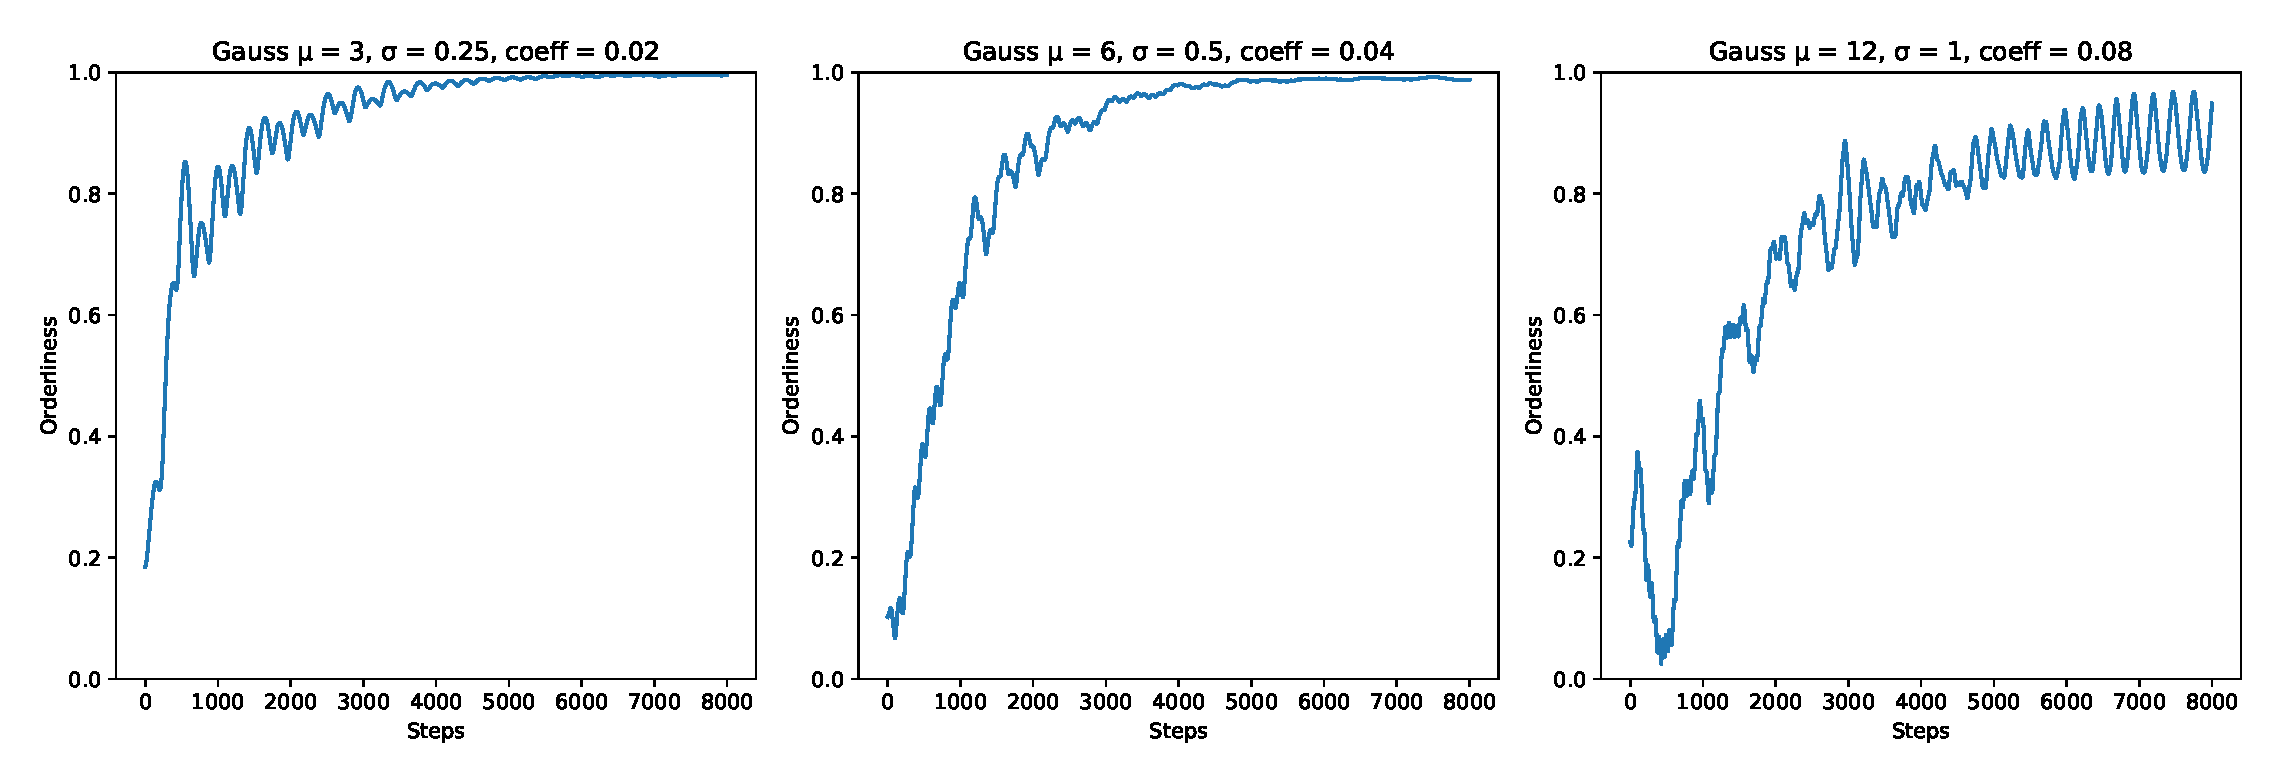
\includegraphics{exp1_freq}}
\caption{Rôzne hodnoty $\sigma$, $\mu$ a coeff \label{Exp1F}}
\end{figure}

Z experimetu je vidno, že nezáleží na počiatočnej frekvencii svetlušiek. Toto tvrdenie by sme nepovažovali za obsolútne, keďže charakteristiky usporiadania simulácií nie sú rovnaké. Ako je možné vidieť v obrázku \ref{Exp1F} pri 3. simulácii dochádza k miernym osciláciam usporiadania. To by sme skôr priradili k artefaktu rozlýšenia simulácie, keďže čím vyššia frekvencia\,-\,tým menej vzorkov na periódu\,-\,tým menej presná simulácia. Preto sa v ďalších simuláciach bude pokračovať výhradne s $\mu = 3$.

\subsection{Experiment 2}
Cieľom experimentu je získať závislosť medzi $\sigma$ normálneho rozdelenia počiatočnej frekvencie a synchronizácie, ktorú tento model nadobudne po určitom počte krokov. Hypotéza je, že s rastúcou $\sigma$ bude postupne klesať zoradenosť systému. Podstatou experimentu je teda iterovať $\sigma$ na určitom intervale bez zmeny ostatných koeficientov a získať priemernú hodnotu zoradenia počas behu programu. Aby sa zamedzilo štatistickým chybám, tak sa pri každej iterácii vykoná simulácia 5x a hodnoty zoradenia sa spriemerujú.

% Vstupy experimentu 2: (nejaka tabulka maybe)
% X = Y patri <2,38> (tj od 4 po 1444 svelušiek)
% coeff patri <0.01, 0.3>
% sigma 3
% mi 0.25
% m 20
% dĺžka behu programu : 12000 krokov

\noindent Vstupy pre experiment 2:
\begin{tabbing}
    X \quad \quad \quad \quad\= Y \quad \quad \quad \quad\= coeff \quad  \quad \quad \quad\= mi \quad  \= s \quad  \quad \quad \quad\= m \quad \= eps \kill %určujem zarážky
    \textbf{X} \> \textbf{Y} \> \textbf{coeff} \> \textbf{$\mu$} \> \textbf{$\sigma$} \> \textbf{m} \> \textbf{$\varepsilon$}\\ 
    $10$          \> $10$    \> $0.02$    \> 3    \> $<$0.01,2$>$     \> 20      \> 0.1  
\end{tabbing}

%(insert image exp1 mi here)
\begin{figure}[h]
    \centering
    \scalebox{0.45}{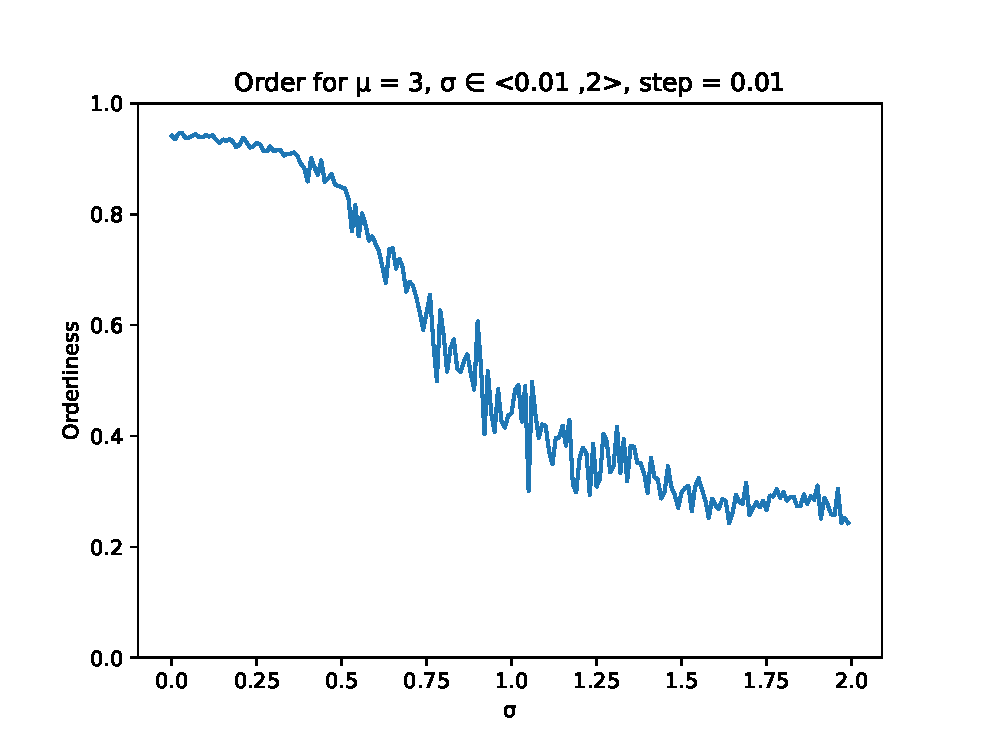
\includegraphics{exp1_mi}}
\caption{Poriadok pri rôznych $\sigma$ \label{Exp1M}}
\end{figure}

Z experimentu vyplýva, že hypotéza bola správna. V ďalších experimentoch budeme pokračovať s hodnotou $\sigma = 0.25$.






\subsection{Experiment 3}
Experiment č. 3 je hlavný experiment tejto štúdie. Cieľom experimentu je pozrieť sa na správanie rôzne velkých skupín svetlušiek pri rôznych hodnotách koeficientu sili viazanosti svetlušiek. 

% Vstupy experimentu 3,a:
% X = Y patri <2,38> (tj od 4 po 1444 svelušiek)
% coeff patri <0.01, 0.3>
% sigma 3
% mi 0.25
% m 20
% dĺžka behu programu : 12000 krokov

\noindent Vstupy pre experiment 3a:
\begin{tabbing}
    X \quad \quad \quad \quad\= Y \quad \quad \quad \quad\= coeff \quad  \quad \quad \quad\= mi \quad  \= s \quad  \quad \= m \quad \= eps \kill %určujem zarážky
    \textbf{X} \> \textbf{Y} \> \textbf{coeff} \> \textbf{$\mu$} \> \textbf{$\sigma$} \> \textbf{m} \> \textbf{$\varepsilon$}\\ 
    $<$2,38$>$          \> $<$2,38$>$    \> $<$0.01,0.3$>$    \> 3    \> 0.25     \> 20      \> 0.1  
\end{tabbing}

Výstup experimentu:
Pre každú kombináciu veľkosti pola a koeficientu sili viazanosti svetlušiek sa získa priemerná hodnota zoradenosti. Pre to aby sa zamedzilo štatistickým chybám z normálneho rozdelenia, tak sa každá simulácia s každým koeficientom pustila 10-krát a výsledky sa spriemerovali. Výstupom je graf na štýl tepelnej mapy, pričom svetlé miesta na grafe značia vysokú synchronizáciu svetlušiek a tmavé malú synchronizáciu svetlušiek.

%(insert experimenty here 3,a a 3b)
% \begin{figure}[h]
%     \centering
%     \scalebox{0.5}{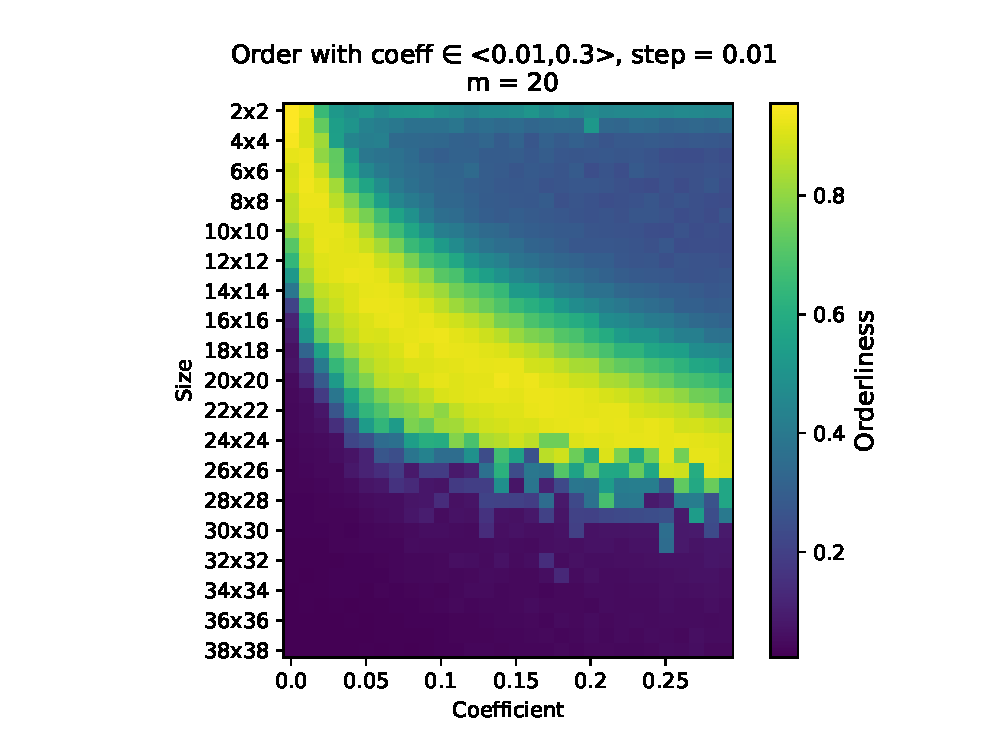
\includegraphics{exp2_2d1}}
% \caption{Poriadok pri rôznych $\sigma$ \label{Exp21}}
% \end{figure}


\begin{figure}
\centering
\begin{minipage}{.5\textwidth}
  \centering
  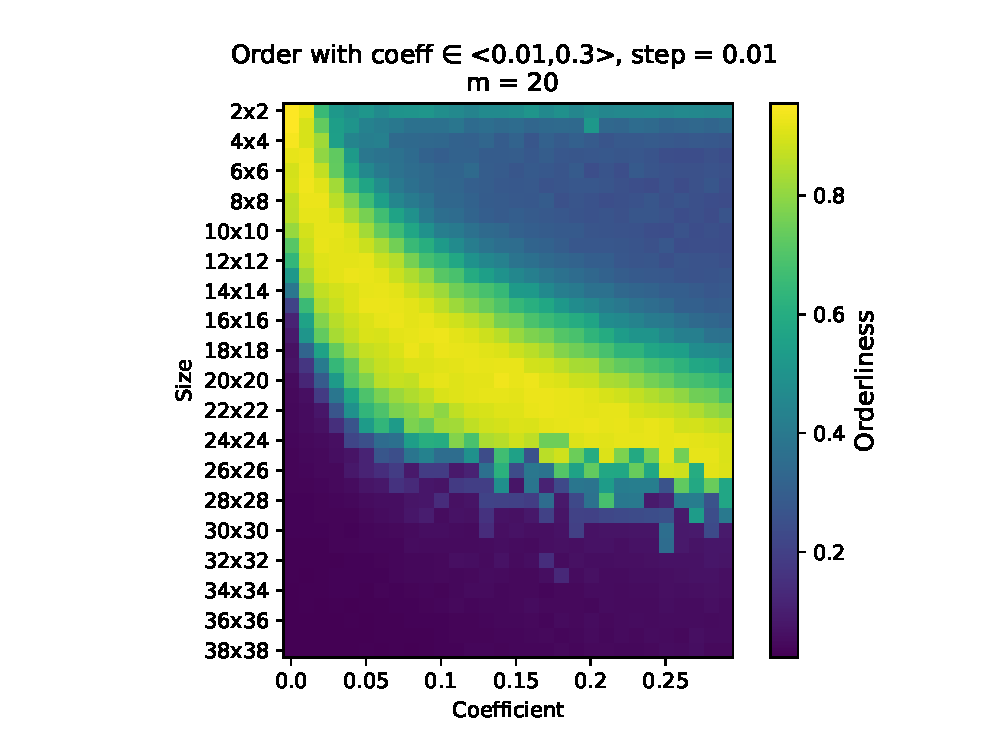
\includegraphics[width=1.1\linewidth]{exp2_2d1}
  \caption{Experiment 3a \label{Exp21}}
\end{minipage}%
\begin{minipage}{.5\textwidth}
  \centering
  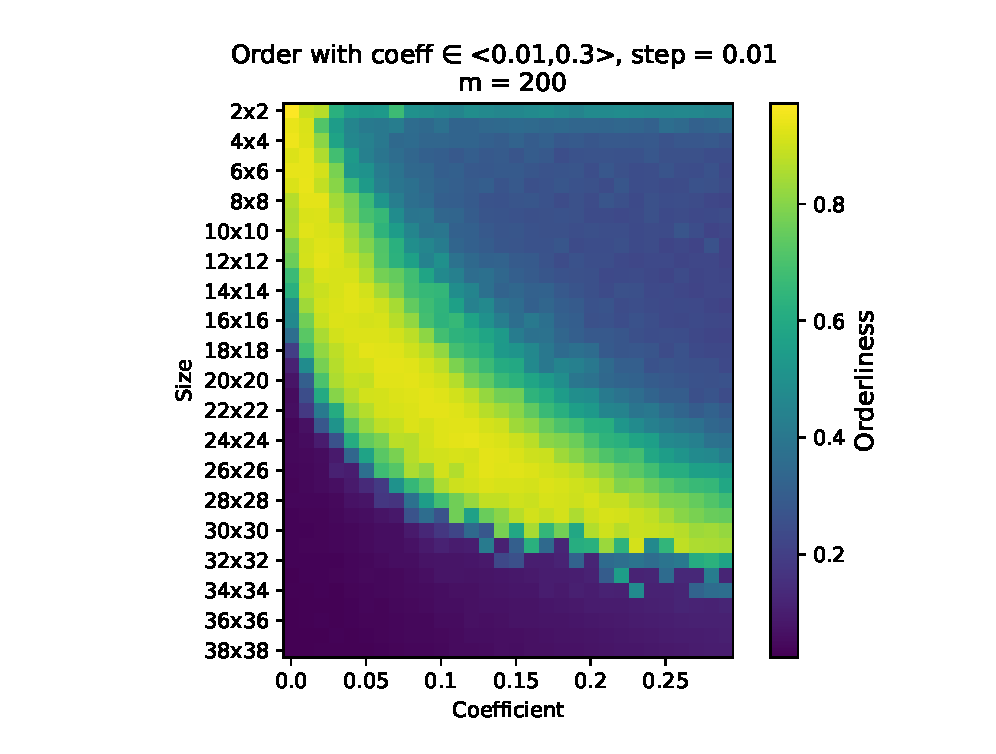
\includegraphics[width=1.1\linewidth]{exp2_2d2}
  \caption{Experiment 3b \label{Exp22}}
\end{minipage}
\end{figure}







Čo je možné pozorovať na experimente 3a je, že svetlušky sa sychronizovali iba do určitého kritického počtu svetlušiek, i keď medzi nimi bola veľká viazanosť. Na základe tohto experimentu sme vykonali ďalší experiment s rovnakými parametrami ale so zmenou parametru m - sila svietenia svetlušky.

% Vstupy experimentu 3,b:
% Okrem m rovnaké ako 3,a
% m 200
\noindent Vstupy pre experiment 3b:
\begin{tabbing}
    X \quad \quad \quad \quad\= Y \quad \quad \quad \quad\= coeff \quad  \quad \quad \quad\= mi \quad  \= s \quad  \quad \= m \quad \= eps \kill %určujem zarážky
    \textbf{X} \> \textbf{Y} \> \textbf{coeff} \> \textbf{$\mu$} \> \textbf{$\sigma$} \> \textbf{m} \> \textbf{$\varepsilon$}\\ 
    $<$2,38$>$          \> $<$2,38$>$    \> $<$0.01,0.3$>$    \> 3    \> 0.25     \> 200      \> 0.1  
\end{tabbing}


V experimente je možné pozorovať, že kritický počet svetlušiek sa posunul z približne 730 (27x27) na 1100 (33x33). Dovolíme si tvrdiť, hoci čerpáme dáta iba z týchto dvoch experimetov, že zo zvyšujúcim sa koeficientom m - koeficient svitu svetlušky - sa budú svetlé miesta na grafe posúvať smerom dole, teda kritický počet svetlušiek sa bude zvyšovať. 

V oboch experimentoch je možné vidieť že svetlušky, najmä pri malých počtoch, sa prestávajú synchronizovať pri zväčšujúcom sa koeficiente a začínajú oscilovať. Toto chovanie bolo už opísané v kapitole \ref{sec_synchron} na obrázku \ref{Order}. Čo je ale zajujímavé na výsledkoch experimetov je to, že sa hranica koeficientu pri ktorom sa prestanú synchronizovať zvyšuje. Toto by sa dalo vysvetliť tým, že systém s menším počtom svetlušiek (oscilátorov) má menší moment energie a tým pádom je náchylnejší na zmeny.

Opak tohto javu je možné pozorovať pri malých koeficientoch a pri zvyšujúcom sa počte svetlušiek. Model so zväčšujúcim sa počtom svetlušiek potrebuje svetlušky s väčším koeficientom viazanosti na to aby sa svetlušky synchronizovali.






\pagebreak 
\section{Záver}
Myslíme si, že sme splnili prvý ciel simulačnej štúdie a to ten, či sa synchronizácia svetlušiek dá modelovať pomocou celuárneho automatu. Taktiež máme za to, že náš model je v istom smere rozšírením štúdie o ktorú sa opierame a to v tom, že svetlušky na seba pôsobia iba v prípade ak zablikajú, a sila akou pôsobia na svoje vnútorné osclátory je ovplivnená aj vzájomnou vzdialenosťou medzi svetluškami.

Z prvých dvoch experimentov vyplývajú celkom priamočiare závery. Nezáleží na frekvencii blikania\\ a čím väčšie sú rozdiely medzi frekvenciami blikania svetlušiek, tým ťažšie sa zosynchronizujú, až sa napokon nezosynchronizujú vôbec.

Z tretieho experimentu vyplýva zaujímavý poznatok, ktorý sme neočakávali a to ten, že svetlušky sa nezosynchronizujú nad istý kritický počet. Naše pôvodné predpoklady boli, že svetlušky sa zosynchronizujú nezávisle na počte, pričom pri veľkých počtoch svetlušiek by vznikali lokálne skupiny zosynchronizovaných svetlušiek a tieto skupiny by sa postupne synchronizovali až pokial by sa nezosinchronizoval celý systém.

% Dodatočný experiment 3,b ukázal že je možné posunúť tento kritický počet tak aby sa zosynchronizovali aj vačší počet svetlušiek a to tak, že zmeníme koeficient svietivosti svetlušky 

Dodatočný experiment 3b ukázal, že je možné posunúť tento kritický počet tak aby sa zosynchronizoval aj väčší počet svetlušiek. To sa teda dá dosiahnuť zväčšením svietivosti svetlušky, čo má za efekt, že jedna svetluška ovplivňuje svetlušky vo väčšej vzdialenosti viac.

Z týchto simulačných experimentov teda vyplýva, že svetlušky \textit{Pteroptyx malaccae} na ktorých bola táto simulačná štúdia založená musia byť evolučne naprogramované tak aby zapadali do svetlej zóny z experimentov 3a a 3b.








\pagebreak



% \begin{algorithm}[h]
% \DontPrintSemicolon
% \SetAlgorithmName{Algoritmus}
% % space necessary

% \IndpD
% \SetNlSty{}{}{}
%     \For{Každá svetluška}{
%         \If{Svetluška zasvietila}{
%             Ovplivni ostatné svetlušky
%         }
        
%     }
% \caption{\textsc{Krok}\label{alg1}}     
% \end{algorithm}

% \begin{figure}[h]
%     \hspace*{-0.8cm}
%     \resizebox{18cm}{12cm}{\includegraphics{kuramoto}}
% \caption{Pic\label{obr1}}
% \end{figure}





\pagebreak
\bibliographystyle{czechiso}
\bibliography{citing}

\end{document}